\documentclass[conference]{IEEEtran}
\IEEEoverridecommandlockouts
% The preceding line is only needed to identify funding in the first footnote. If that is unneeded, please comment it out.
\usepackage{cite}
\usepackage{amsmath,amssymb,amsfonts}
\usepackage{algorithmic}
\usepackage{graphicx}
\usepackage{textcomp}
\usepackage{xcolor}
\usepackage{hyperref}
\usepackage{multirow}
\def\BibTeX{{\rm B\kern-.05em{\sc i\kern-.025em b}\kern-.08em
    T\kern-.1667em\lower.7ex\hbox{E}\kern-.125emX}}
\begin{document}

\title{Automated Detection of Brain Tumor and Brain Stroke}

% \author{\IEEEauthorblockN{1\textsuperscript{st} Given Name Surname}
% \IEEEauthorblockA{\textit{dept. name of organization (of Aff.)} \\
% \textit{name of organization (of Aff.)}\\
% City, Country \\
% email address or ORCID}
% \and
% \IEEEauthorblockN{2\textsuperscript{nd} Given Name Surname}
% \IEEEauthorblockA{\textit{dept. name of organization (of Aff.)} \\
% \textit{name of organization (of Aff.)}\\
% City, Country \\
% email address or ORCID}
% \and
% \IEEEauthorblockN{3\textsuperscript{rd} Given Name Surname}
% \IEEEauthorblockA{\textit{dept. name of organization (of Aff.)} \\
% \textit{name of organization (of Aff.)}\\
% City, Country \\
% email address or ORCID}
% \and
% \IEEEauthorblockN{4\textsuperscript{th} Given Name Surname}
% \IEEEauthorblockA{\textit{dept. name of organization (of Aff.)} \\
% \textit{name of organization (of Aff.)}\\
% City, Country \\
% email address or ORCID}
% \and
% \IEEEauthorblockN{5\textsuperscript{th} Given Name Surname}
% \IEEEauthorblockA{\textit{dept. name of organization (of Aff.)} \\
% \textit{name of organization (of Aff.)}\\
% City, Country \\
% email address or ORCID}
% \and
% \IEEEauthorblockN{6\textsuperscript{th} Given Name Surname}
% \IEEEauthorblockA{\textit{dept. name of organization (of Aff.)} \\
% \textit{name of organization (of Aff.)}\\
% City, Country \\
% email address or ORCID}
% }

\maketitle


%%%%%%%%%%%%%%%%%%%%%%%%%%%%%%%%%%%%%%%%%%%%%%%%%%%%%%%%%%%%%%%%%%%%%%%%%%%%%%%%
\begin{abstract}

Automated detection of brain tumors and strokes from medical images can help improve diagnosis and treatment, especially in resource-constrained settings where there may be shortages of specialized radiologists and neurologists.
Manual analysis of scans by experts is time-consuming and its availability depends on their schedules. This often leads to treatment delays for patients. 
Common techniques for the detection of brain abnormalities rely on manual segmentation and feature extraction from images by radiologists. Recently, deep learning methods like Convolutional Neural Networks (CNNs) have shown promising performance in various medical image analysis tasks.

However, applying these techniques requires large, annotated datasets which are challenging to obtain due to the expertise required for labeling. In this research, the aim is to develop a website for detecting brain tumors and strokes from MRI scans to assist intensive care physicians.

Around 3000 MRI images were collected from public datasets and dataset settings to facilitate model training and due to the large dataset size, the model training process is divided into phases. 

There are two classes in the dataset: positive (tumor present) and negative (no tumor).

\end{abstract}

\begin{IEEEkeywords}
brain tumor, brain stroke, CV
\end{IEEEkeywords}


%%%%%%%%%%%%%%%%%%%%%%%%%%%%%%%%%%%%%%%%%%%%%%%%%%%%%%%%%%%%%%%%%%%%%%%%%%%%%%%%
\section{INTRODUCTION}

Brain tumors, whether malignant or benign, pose a severe threat due to their growth in or near the brain, affecting vital functions (Figure \ref{fig:brain_with_tumor}) \cite{br35h}. Accurate classification aids in early diagnosis, necessitating optimized digital methods like deep learning models from MRI data \cite{bioengineering9120783}.

Stroke, a sudden interruption of blood flow to the brain, is a leading cause of death and disability worldwide. Timely intervention, including reperfusion therapy, is crucial for salvaging ischemic brain tissue and improving post-stroke outcomes. Utilizing a CNN model, multi-image classification categorizes MRI scans into tumor, no tumor, stroke, or normal, facilitating timely diagnosis and treatment decisions \cite{huggingface_data, ding2021repvgg}.

Brain tumors are the growth of abnormal cells in or near brain tissue and are considered one of the most important and dangerous brain diseases. In the early stages, they can often be removed with surgery leading to complete recovery. However, in advanced stages, complete recovery becomes less likely. As a result, the average 5-year survival rate for those diagnosed in the early stages is about 92\%, while it drops to approximately 36\% for those diagnosed at a later stage \cite{Kang2023, kang2023bgfyolo}.

\begin{figure}
    \centering
    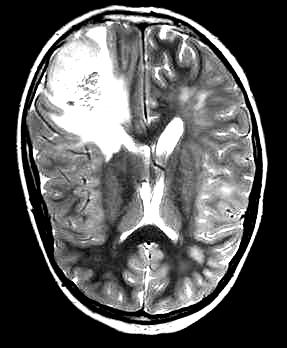
\includegraphics[scale=0.5]{figures/brain_with_tumor.jpg}
    \caption{Human Brain Affected With Tumor \cite{br35h}}
    \label{fig:brain_with_tumor}
\end{figure}

A stroke happens when blood flow to any part of the brain stops. Each person has a different recovery time and need for long-term care. Problems with moving, thinking, and talking often improve in the first weeks or months after a stroke. Some people will continue to improve months or even years after a stroke \cite{jocher2022yolo5, iandola2014densenet}. Artificial intelligence has proven its superiority in detecting diseases using MRI and CT scans \cite{ABDELMAKSOUD201571-51, chen791-53}.

We have designed a program specifically to assist healthcare professionals and patients in diagnosing and detecting brain diseases. One challenge we face is developing a model that achieves satisfactory results. Another challenge is designing a user interface suitable for all users, whether they are doctors, nurses, or patients. Despite these challenges, we have achieved satisfactory results according to our clients.

The objective of this project is to help patients and intensive care doctors detect brain tumors and stroke easily from MRI and CT scans. We will use artificial intelligence, machine learning, and neural network techniques to detect brain strokes and tumors. Our goal is to build an accessible website for both patients and doctors that will assist in providing accurate diagnoses \cite{ma82, dattaad:10.1504}.

\section{ RELATED WORK}

% In this section, we study previous research works about brain tumor and brain stroke detection using the CNN algorithm. we design two models one for brain tumors and another for brain stroke.

Recent advancements in machine learning and deep learning have significantly impacted the field of medical imaging, particularly in brain tumor detection and segmentation. Numerous studies have explored different approaches to enhance the accuracy and efficiency of these processes.

Ahmed Hamada's dataset, \emph{Br35H:: Brain Tumor Detection 2020}, available on Kaggle, provides a comprehensive set of MRI images for brain tumor detection, facilitating the development and benchmarking of various algorithms \cite{br35h}. Similarly, the \emph{MRI-Images-of-Brain-Tumor} dataset on Huggingface by PranomVignesh serves as a valuable resource for training and evaluating deep learning models in this domain \cite{huggingface_data}.

Object detection models like YOLO (You Only Look Once) have been adapted for medical image analysis. The configurations for YOLOv7 \cite{wong2020yolo7} and YOLOv5 \cite{jocher2022yolo5} have been documented on GitHub, highlighting their potential for fast and accurate detection of brain tumors. Kang et al. introduced RCS-YOLO, a high-accuracy object detector specifically designed for brain tumor detection, demonstrating its effectiveness in clinical settings \cite{Kang2023}. Additionally, the BGF-YOLO model enhances YOLOv8 with multiscale attentional feature fusion, further improving detection performance \cite{kang2023bgfyolo}.

Convolutional neural networks (CNNs) have also shown promise in medical image segmentation. The RepVGG model by Ding et al. proposes a VGG-style ConvNet that balances simplicity and performance \cite{ding2021repvgg}. DenseNet, introduced by Iandola et al., implements efficient ConvNet descriptor pyramids, optimizing feature reuse and network efficiency \cite{iandola2014densenet}.

Hybrid clustering techniques have been employed to improve brain tumor segmentation. Abdel-Maksoud et al. developed a method combining K-means clustering with Fuzzy C-means and level set segmentation, achieving high accuracy and efficiency \cite{ABDELMAKSOUD201571-51}. Similarly, Beddad et al. presented a cooperative approach integrating K-means and fuzzy clustering for MRI image segmentation \cite{dattaad:10.1504}.

Advanced decision support systems leverage deep learning for automated medical diagnostics. Masood et al. proposed an enhanced region-based fully convolutional network (RFCN) with multilayer fusion for lung cancer detection, showcasing its applicability in other medical fields such as brain tumor detection \cite{masood900}. 

Chen et al. explored disease prediction using big data and machine learning, emphasizing the importance of comprehensive data management practices for accurate medical analytics \cite{chen791-53}. This is further supported by the findings of Munappy et al., who identified data management challenges in deep learning workflows for medical applications \cite{munppy89-16}.

Lastly, Ma et al. introduced a multiscale patch-driven active contour model combined with random forests for automated brain tumor segmentation, demonstrating significant improvements in segmentation accuracy \cite{ma82}.

These studies collectively highlight the potential of combining advanced machine learning techniques with robust data management practices to improve brain tumor detection and segmentation accuracy and efficiency.

\section{WORK SCOPE}
 Today's ailments are on the rise due to our hectic and stressful lifestyles. All age groups are susceptible to illness, thus early detection is critical. Pneumonia, lung cancer, and brain tumor diseases by using symptoms or reports. Most people throughout the world still lack access to the necessary instruments for the early identification of these illnesses. One of the most hazardous diseases among both genders, early diagnosis and treatment are critical to the health of those sick. For the future, we're going to invent a strong system that can accurately work on a large medical dataset with several lung cancer and brain tumor diseases.
 

\section{ PURPOSED SYSTEM}

Begin by laying out the model structure using layers such as convolutional, batch normalization, activation, and max pooling to derive attributes from the inputted images. Incorporate a flattened layer to transform the resulting data from the convolutional core to a 1D vector.
Integrate fully connected layers to facilitate classification. Set up the model by designating loss function, optimizer, and metrics. Establish callbacks such as TensorBoard for the purpose of logging, and ModelCheckpoint to retain the optimal model weights. Divvy up the dataset into training and validation groups using a function designed for data splitting. 

Iteratively process the training data in batches: Train the model on a batch with the history noted Assess the model using the validation set Retain model checkpoints based on validation loss. For the proposed system, the TensorFlow and Keras frameworks were used to build the deep learning model. 

An intuitive user interface was developed using Figma\footnote{\url{https://figma.com}} for healthcare professionals to obtain results easily. 
The proposed models achieved 92\% and 90\% accuracy on test data for binary classification of normal vs abnormal scans. The system helps to solve the issue of time taken for specialists to diagnose brain conditions from scans. 

\subsection{SYSTEM ARCHITECTURE}

The architecture of the proposed system design is illustrated in Figure \ref{fig:sys_arch}.

\begin{figure}
    \centering
    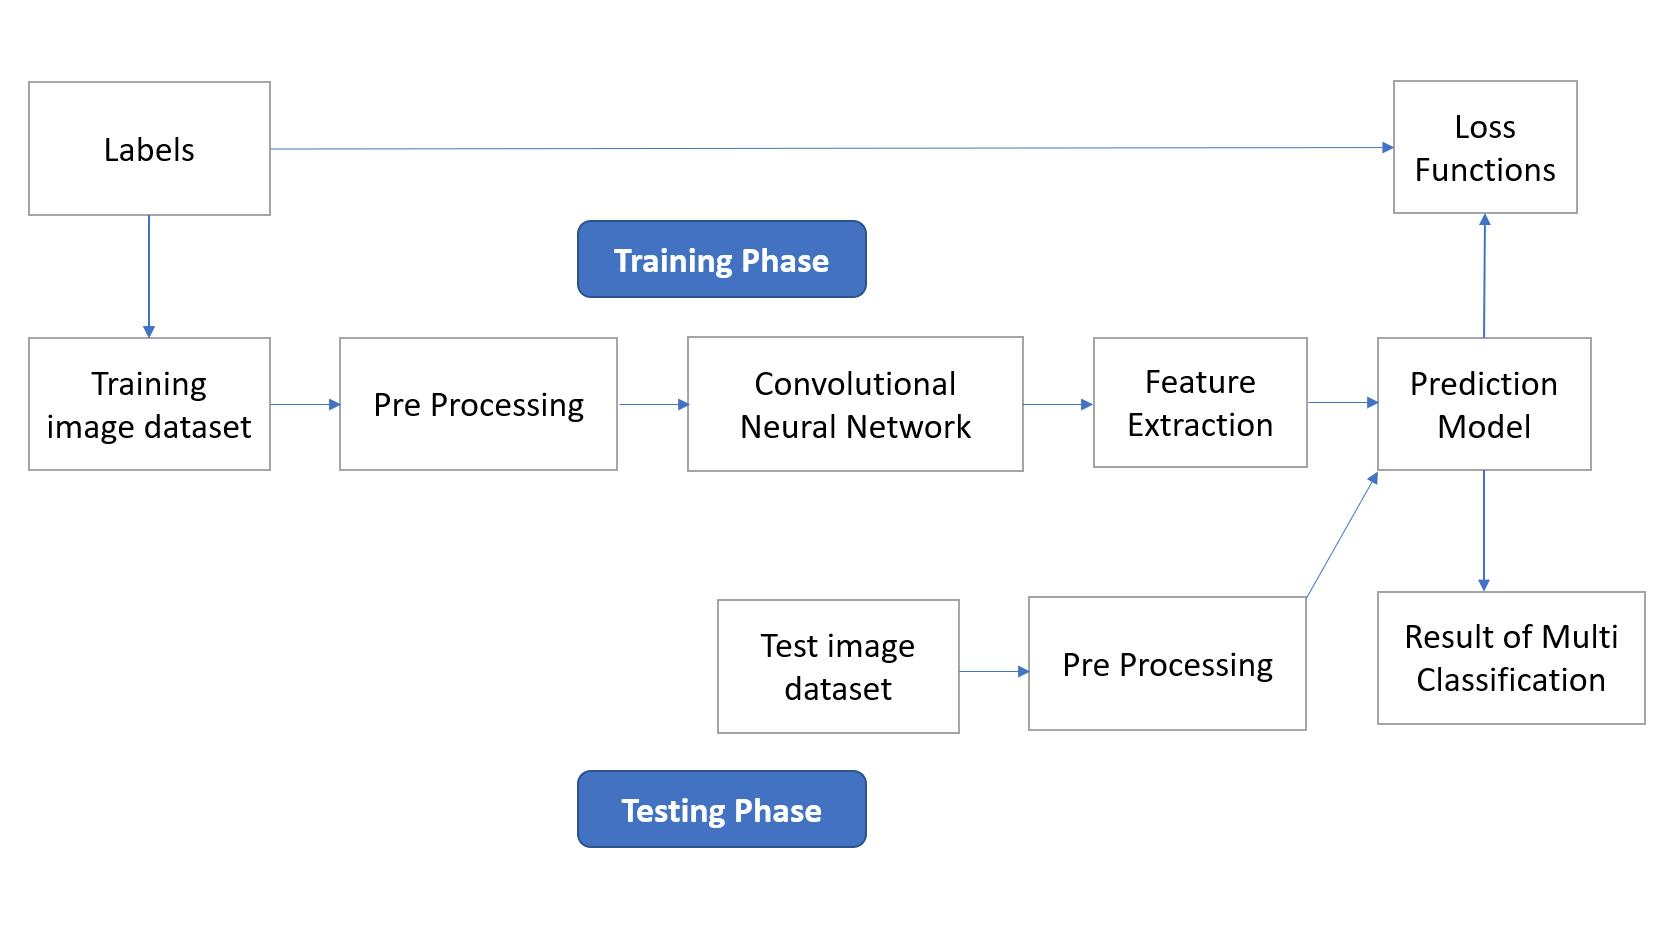
\includegraphics[width=0.45\textwidth]{figures/9.jpg}
    \caption{System Architecture}
    \label{fig:sys_arch}
\end{figure}

\subsubsection{Processing Steps}

The initial step in the pipeline is pre-processing, which adapts the images according to the requirements of subsequent stages. This process includes noise reduction, edge sharpening, and conversion from RGB to grayscale. A median filter is utilized for noise removal, although modern MRI scans typically exhibit low noise levels.

\subsubsection{Approximate Reasoning}

To estimate the tumor size, a linearization approach is employed as the first stage of deductive reasoning. This involves converting the image to a binary format, where the pixels are either black or white (0 or 1). Following this, the tumor stage is defined, and its prognosis is forecasted based on the identified tumor area.

\subsection{Models Architecture}

\subsubsection{Brain Tumor Detection}

\paragraph{Dataset}

For brain tumor detection, we utilize two primary datasets: Br35H \cite{br35h} for training and a dataset from Huggingface \cite{huggingface_data} for testing. These datasets comprise various brain MRI images categorized into negative (no tumor) and positive (tumor) samples.

\paragraph{Data Shuffling and Splitting}
Samples are shuffled, and if the total number exceeds the limit, they are either split into chunks or truncated to optimize learning performance.

\paragraph{Cropping}
To enhance detection accuracy, we focus on the region of interest (ROI), specifically the brain. A cropping technique isolates the brain by identifying the extreme points of the brain contour using OpenCV.

\subsubsection{Image Preparation and Resizing}
Images are loaded and preprocessed by cropping the brain region, resizing to the desired dimensions, and normalizing. Sample images are visualized to ensure correct preprocessing.

\subsubsection{Model Training}
The dataset is divided into training and test sets. The model undergoes training and monitoring using various metrics. Callbacks are employed to save the best model, and the training process is logged for subsequent analysis. Performance is evaluated on the test set, with additional metrics such as the F1 score to assess effectiveness.

\subsection{Brain Stroke Detection}

For brain stroke detection, we utilized a private dataset from a local hospital. This dataset includes a variety of brain MRI images categorized into negative (no stroke) and positive (stroke) samples.

\paragraph{Image Preprocessing}
Functions are implemented for resizing, normalizing, and merging image slices into 3D scans.

\paragraph{Dataset Loading}
The entire dataset is loaded into memory as a 4D array, labeled as stroke (1) or normal (0), and divided into training and validation sets.

\subsubsection{Model Architecture and Training}

\paragraph{Model Architecture}
The architecture of the 3D Convolutional Neural Network (CNN) model incorporates augmentation layers. The model is compiled with appropriate loss functions, optimizers, and performance metrics.

\paragraph{Model Training and Evaluation}
This final step involves setting up callbacks for saving the best model, defining the training function, and training the model with various augmentation strategies. The training process is conducted over 150 epochs (EPOCHS = 150), ensuring thorough evaluation and performance optimization.

 
\section{RESULTS AND DISCUSSION}

In this work, we developed and evaluated models for detecting brain tumors and strokes using MRI and CT scan images, respectively. Our approach leveraged advanced convolutional neural networks (CNNs) and comprehensive data preprocessing techniques to achieve significant results. The brain tumor detection model achieved an accuracy of 92\%, while the brain stroke detection model reached an accuracy of 90\%. These results demonstrate the effectiveness of our models in medical image analysis.

Despite these promising outcomes, there is room for improvement. Enhancing model performance could be achieved by incorporating additional data, which would provide a more extensive training set and help the model generalize better to unseen cases. Future work will focus on:
\begin{itemize}
    \item Expanding the dataset with more diverse and comprehensive samples.
    \item Exploring data augmentation techniques to artificially increase the dataset size.
    \item Implementing advanced deep learning architectures and techniques to further boost accuracy and robustness.
\end{itemize}

By addressing these areas, we aim to develop even more reliable and accurate models for brain tumor and stroke detection, ultimately contributing to better diagnostic tools in healthcare.

Table \ref{tab:brain_tumor_comparison} compares the accuracy of our brain tumor detection model with other recent studies. As shown, our model performs competitively, but there is still potential for improvement by leveraging larger and more diverse datasets, as well as advanced machine learning techniques.

\begin{table}[htbp]
\caption{Comparison With Other Brain Tumor Detection Papers}
\begin{center}
\begin{tabular}{|p{2cm}|p{4cm}|c|}
\hline
\textbf{Name} & \textbf{Dataset Description} & \textbf{Accuracy} \\
\hline
BGF-YOLO \cite{kang2023bgfyolo} & Classes: Tumor, no Tumor \newline Dataset: 804 images \newline Training: 501 \newline Validation: 202 \newline Testing: 101 & 91\% \\
\hline
RCS-YOLO \cite{wong2020yolo7} & Classes: Tumor, no Tumor \newline Dataset \cite{br35h}: 701 images \newline Training: 500 \newline Validation: 202 & 90\% \\
\hline
\emph{The proposed model} & Classes: Tumor, Normal \newline Dataset: 3000 images & 92\% \\
\hline
\end{tabular}
\label{tab:brain_tumor_comparison}
\end{center}
\end{table}

Similarly, Table \ref{tab:brain_stroke_comparison} compares the accuracy of our brain stroke detection model with other recent studies. Our model shows promising results but indicates that further enhancements could be made by employing larger datasets and more sophisticated algorithms.

\begin{table}[htbp]
\caption{Comparison With Other Brain Stroke Detection Papers}
\begin{center}
\begin{tabular}{|p{2cm}|p{4cm}|c|}
\hline
\textbf{Name} & \textbf{Dataset Description} & \textbf{Accuracy} \\
\hline
OzNet \cite{bioengineering9120783} & Classes: Stroke, Normal \newline Dataset: 1900 images & 87.47\% \\
\hline
OzNet-mRMR-NB \cite{bioengineering9120783} & Classes: Stroke, Normal \newline Dataset: 1900 images & 98.42\% \\
\hline
\emph{The proposed model} & Classes: Stroke, Normal \newline Dataset: 1000 images & 90\% \\
\hline
\end{tabular}
\label{tab:brain_stroke_comparison}
\end{center}
\end{table}

The tables illustrate that while our models are competitive, there is still significant potential for improvement. Incorporating larger and more diverse datasets, utilizing advanced machine learning techniques, and further optimizing our CNN architectures could enhance the accuracy and robustness of our models. This work represents a step towards more effective diagnostic tools in healthcare, ultimately contributing to improved patient outcomes.



\section{CONCLUSION}

This research has demonstrated the potential of convolutional neural networks (CNNs) for detecting brain tumors and strokes using MRI and CT scan images, respectively. By employing advanced data preprocessing techniques and robust model architectures, we achieved notable accuracies of 92\% for brain tumor detection \cite{br35h} and 90\% for stroke detection \cite{bioengineering9120783}. These results underscore the effectiveness of our approach in enhancing medical image analysis.

Our comprehensive approach, encompassing dataset preparation, model training, and evaluation, ensures that healthcare professionals can rely on these models for accurate and timely diagnoses. The implementation of an intuitive user interface further facilitates the practical application of these models in clinical settings, making advanced diagnostic tools more accessible.

Ultimately, our goal is to provide healthcare professionals with reliable diagnostic tools that improve patient outcomes by enabling timely and accurate medical care. Future work will focus on refining our models by incorporating larger and more diverse datasets, exploring innovative data augmentation techniques \cite{huggingface_data}, and implementing cutting-edge deep learning architectures. By continuing to enhance and expand our models, we aim to make a significant contribution to the advancement of medical diagnostics and patient care.

\section{FUTURE WORK}

Future work involves collecting additional real-world data and exploring explainable models to increase the accuracy of brain tumor and brain stroke detection. 
The goal is to provide timely diagnoses and treatment to improve patient outcomes.
So the goal of the project is to help doctors and patients get Proper medical care.

 

%%%%%%%%%%%%%%%%%%%%%%%%%%%%%%%%%%%%%%%%%%%%%%%%%%%%%%%%%%%%%%%%%%%%%%%%%%%%%%%
% Bibliography
%%%%%%%%%%%%%%%%%%%%%%%%%%%%%%%%%%%%%%%%%%%%%%%%%%%%%%%%%%%%%%%%%%%%%%%%%%%%%%%

% \begin{thebibliography}{00}
% \bibliography{refs.bib} % INCLUDE: Bibliography file
% \end{thebibliography}

% The bibliography section
\begin{thebibliography}{00}

\bibitem{bioengineering9120783}
Oznur Ozaltin, Orhan Coskun, Ozgur Yeniay, Abdulhamit Subasi,
\emph{A Deep Learning Approach for Detecting Stroke from Brain CT Images Using OzNet},
Bioengineering,
2022.
\url{https://www.mdpi.com/2306-5354/9/12/783}

\bibitem{br35h}
Ahmed Hamada,
\emph{Br35H :: Brain Tumor Detection 2020},
Kaggle,
2020.
\url{https://www.kaggle.com/datasets/ahmedhamada0/brain-tumor-detection}

\bibitem{huggingface_data}
PranomVignesh,
\emph{MRI-Images-of-Brain-Tumor},
Huggingface,
2023.
\url{https://huggingface.co/datasets/PranomVignesh/MRI-Images-of-Brain-Tumor}

\bibitem{wong2020yolo7}
Kin-Yiu Wong,
\emph{Yolov7.yaml},
GitHub,
2020.
\url{https://github.com/WongKinYiu/yolov7/blob/main/cfg/training/yolov7.yaml}

\bibitem{jocher2022yolo5}
Glenn Jocher,
\emph{YOLOv5 (6.0/6.1) brief summary},
GitHub,
2022.
\url{https://github.com/ultralytics/yolov5/issues/6998}

\bibitem{Kang2023}
Ming Kang and Chee-Ming Ting and Fung Fung Ting and Raphaël C.-W. Phan,
\emph{RCS-YOLO: A Fast and High-Accuracy Object Detector for Brain Tumor Detection},
Lecture Notes in Computer Science,
Springer Nature Switzerland,
2023,
pp. 600-610.
\url{https://doi.org/10.1007%2F978-3-031-43901-8_57}

\bibitem{kang2023bgfyolo}
Ming Kang and Chee-Ming Ting and Fung Fung Ting and Raphaël C. -W. Phan,
\emph{BGF-YOLO: Enhanced YOLOv8 with Multiscale Attentional Feature Fusion for Brain Tumor Detection},
2023.
\url{https://arxiv.org/abs/2309.12585}

\bibitem{ding2021repvgg}
Xiaohan Ding and Xiangyu Zhang and Ningning Ma and Jungong Han and Guiguang Ding and Jian Sun,
\emph{RepVGG: Making VGG-style ConvNets Great Again},
2021.
\url{https://arxiv.org/abs/2101.03697}

\bibitem{iandola2014densenet}
Forrest Iandola and Matt Moskewicz and Sergey Karayev and Ross Girshick and Trevor Darrell and Kurt Keutzer,
\emph{DenseNet: Implementing Efficient ConvNet Descriptor Pyramids},
2014.
\url{https://arxiv.org/abs/1404.1869}

\bibitem{rowling1997}
J.K. Rowling,
\emph{Harry Potter and the Philosopher's Stone},
Bloomsbury,
1997.

\bibitem{ma82}
Chao Ma and Gongning Luo and Kuanquan Wang,
\emph{Concatenated and Connected Random Forests With Multiscale Patch Driven Active Contour Model for Automated Brain Tumor Segmentation of MR Images},
IEEE Transactions on Medical Imaging,
2018,
vol. 37, no. 8, pp. 1943-1954.
\url{https://doi.org/10.1109/TMI.2018.2805821}

\bibitem{dattaad:10.1504}
Boucif Beddad and Kaddour Hachemi and Sundarapandian Vaidyanathan,
\emph{Design and implementation of a new cooperative approach to brain tumour identification from MRI images},
International Journal of Computer Applications in Technology,
2019,
vol. 59, no. 1, pp. 1-10.
\url{https://www.inderscienceonline.com/doi/abs/10.1504/IJCAT.2019.097113}

\bibitem{masood900}
Anum Masood and Bin Sheng and Po Yang and Ping Li and Huating Li and Jinman Kim and David Dagan Feng,
\emph{Automated Decision Support System for Lung Cancer Detection and Classification via Enhanced RFCN With Multilayer Fusion RPN},
IEEE Transactions on Industrial Informatics,
2020,
vol. 16, no. 12, pp. 7791-7801.
\url{https://doi.org/10.1109/TII.2020.2972918}

\bibitem{XIA20-15}
Yufei Xia and Chuanzhe Liu and YuYing Li and Nana Liu,
\emph{A boosted decision tree approach using Bayesian hyper-parameter optimization for credit scoring},
Expert Systems with Applications,
2017,
vol. 78, pp. 225-241.
\url{https://www.sciencedirect.com/science/article/pii/S0957417417301008}

\bibitem{munppy89-16}
Aiswarya Munappy and Jan Bosch and Helena Holmström Olsson and Anders Arpteg and Björn Brinne,
\emph{Data Management Challenges for Deep Learning},
2019 45th Euromicro Conference on Software Engineering and Advanced Applications (SEAA),
2019,
pp. 140-147.
\url{https://doi.org/10.1109/SEAA.2019.00030}

\bibitem{ABDELMAKSOUD201571-51}
Eman Abdel-Maksoud and Mohammed Elmogy and Rashid Al-Awadi,
\emph{Brain tumor segmentation based on a hybrid clustering technique},
Egyptian Informatics Journal,
2015,
vol. 16, no. 1, pp. 71-81.
\url{https://www.sciencedirect.com/science/article/pii/S1110866515000043}

\bibitem{chen791-53}
Min Chen and Yixue Hao and Kai Hwang and Lu Wang and Lin Wang,
\emph{Disease Prediction by Machine Learning Over Big Data From Healthcare Communities},
IEEE Access,
2017,
vol. 5, pp. 8869-8879.
\url{https://doi.org/10.1109/ACCESS.2017.2694446}

\bibitem{mohapatra-54}
Hitesh Mohapatra and Amiya Rath,
\emph{Fundamentals of Software Engineering: Designed to provide an insight into the software engineering concepts},
2020,
ISBN: 9388511778, 9789388511773.

\end{thebibliography}

\end{document}
